\begin{figure}[h]
\begin{center}
\begin{adjustbox}{width=\columnwidth}

\tikzset {_tol09vz9c/.code = {\pgfsetadditionalshadetransform{ \pgftransformshift{\pgfpoint{0 bp } { 0 bp }  }  \pgftransformrotate{0 }  \pgftransformscale{2 }  }}}
\pgfdeclarehorizontalshading{_j7rsmr3nr}{150bp}{rgb(0bp)=(0.93,0.93,0.93);
rgb(37.5bp)=(0.93,0.93,0.93);
rgb(62.5bp)=(1,0,0);
rgb(100bp)=(1,0,0)}
\tikzset{_yxq6cdpsj/.code = {\pgfsetadditionalshadetransform{\pgftransformshift{\pgfpoint{0 bp } { 0 bp }  }  \pgftransformrotate{0 }  \pgftransformscale{2 } }}}
\pgfdeclarehorizontalshading{_7yg524gtp} {150bp} {color(0bp)=(transparent!75);
color(37.5bp)=(transparent!75);
color(62.5bp)=(transparent!75);
color(100bp)=(transparent!75) } 
\pgfdeclarefading{_y4z1b8bbb}{\tikz \fill[shading=_7yg524gtp,_yxq6cdpsj] (0,0) rectangle (50bp,50bp); } 

% Gradient Info
  
\tikzset {_3ywdqyfah/.code = {\pgfsetadditionalshadetransform{ \pgftransformshift{\pgfpoint{0 bp } { 0 bp }  }  \pgftransformrotate{0 }  \pgftransformscale{2 }  }}}
\pgfdeclarehorizontalshading{_2t0kw1fpw}{150bp}{rgb(0bp)=(1,0,0);
rgb(37.5bp)=(1,0,0);
rgb(62.5bp)=(0,0,1);
rgb(100bp)=(0,0,1)}
\tikzset{_yvsljnreh/.code = {\pgfsetadditionalshadetransform{\pgftransformshift{\pgfpoint{0 bp } { 0 bp }  }  \pgftransformrotate{0 }  \pgftransformscale{2 } }}}
\pgfdeclarehorizontalshading{_fpvhgjdei} {150bp} {color(0bp)=(transparent!75);
color(37.5bp)=(transparent!75);
color(62.5bp)=(transparent!75);
color(100bp)=(transparent!75) } 
\pgfdeclarefading{_y32y00acn}{\tikz \fill[shading=_fpvhgjdei,_yvsljnreh] (0,0) rectangle (50bp,50bp); } 

% Gradient Info
  
\tikzset {_k82gbaai2/.code = {\pgfsetadditionalshadetransform{ \pgftransformshift{\pgfpoint{0 bp } { 0 bp }  }  \pgftransformrotate{0 }  \pgftransformscale{2 }  }}}
\pgfdeclarehorizontalshading{_mzd6axxaa}{150bp}{rgb(0bp)=(0,0,1);
rgb(37.5bp)=(0,0,1);
rgb(62.5bp)=(0,0,1);
rgb(100bp)=(0,0,1)}
\tikzset{_1ih9fwhej/.code = {\pgfsetadditionalshadetransform{\pgftransformshift{\pgfpoint{0 bp } { 0 bp }  }  \pgftransformrotate{0 }  \pgftransformscale{2 } }}}
\pgfdeclarehorizontalshading{_py52u7ab2} {150bp} {color(0bp)=(transparent!75);
color(37.5bp)=(transparent!75);
color(62.5bp)=(transparent!50);
color(100bp)=(transparent!50) } 
\pgfdeclarefading{_wr0vkxl3y}{\tikz \fill[shading=_py52u7ab2,_1ih9fwhej] (0,0) rectangle (50bp,50bp); } 

% Gradient Info
  
\tikzset {_3kvg59946/.code = {\pgfsetadditionalshadetransform{ \pgftransformshift{\pgfpoint{0 bp } { 0 bp }  }  \pgftransformrotate{-90 }  \pgftransformscale{2 }  }}}
\pgfdeclarehorizontalshading{_wvh4fdo7p}{150bp}{rgb(0bp)=(1,0,0);
rgb(37.5bp)=(1,0,0);
rgb(62.5bp)=(0,0,1);
rgb(100bp)=(0,0,1)}
\tikzset{_dv8t3n3dv/.code = {\pgfsetadditionalshadetransform{\pgftransformshift{\pgfpoint{0 bp } { 0 bp }  }  \pgftransformrotate{-90 }  \pgftransformscale{2 } }}}
\pgfdeclarehorizontalshading{_abfcxja44} {150bp} {color(0bp)=(transparent!75);
color(37.5bp)=(transparent!75);
color(62.5bp)=(transparent!75);
color(100bp)=(transparent!75) } 
\pgfdeclarefading{_tndnn1d2b}{\tikz \fill[shading=_abfcxja44,_dv8t3n3dv] (0,0) rectangle (50bp,50bp); } 

% Gradient Info
  
\tikzset {_475pso13i/.code = {\pgfsetadditionalshadetransform{ \pgftransformshift{\pgfpoint{0 bp } { 0 bp }  }  \pgftransformrotate{-90 }  \pgftransformscale{2 }  }}}
\pgfdeclarehorizontalshading{_f5gjc5tzr}{150bp}{rgb(0bp)=(0,0,1);
rgb(37.5bp)=(0,0,1);
rgb(62.5bp)=(1,0,0);
rgb(100bp)=(1,0,0)}
\tikzset{_fwuteqqte/.code = {\pgfsetadditionalshadetransform{\pgftransformshift{\pgfpoint{0 bp } { 0 bp }  }  \pgftransformrotate{-90 }  \pgftransformscale{2 } }}}
\pgfdeclarehorizontalshading{_gbjam9yyh} {150bp} {color(0bp)=(transparent!75);
color(37.5bp)=(transparent!75);
color(62.5bp)=(transparent!75);
color(100bp)=(transparent!75) } 
\pgfdeclarefading{_wo5obn5gu}{\tikz \fill[shading=_gbjam9yyh,_fwuteqqte] (0,0) rectangle (50bp,50bp); } 
\tikzset{every picture/.style={line width=0.75pt}} %set default line width to 0.75pt        

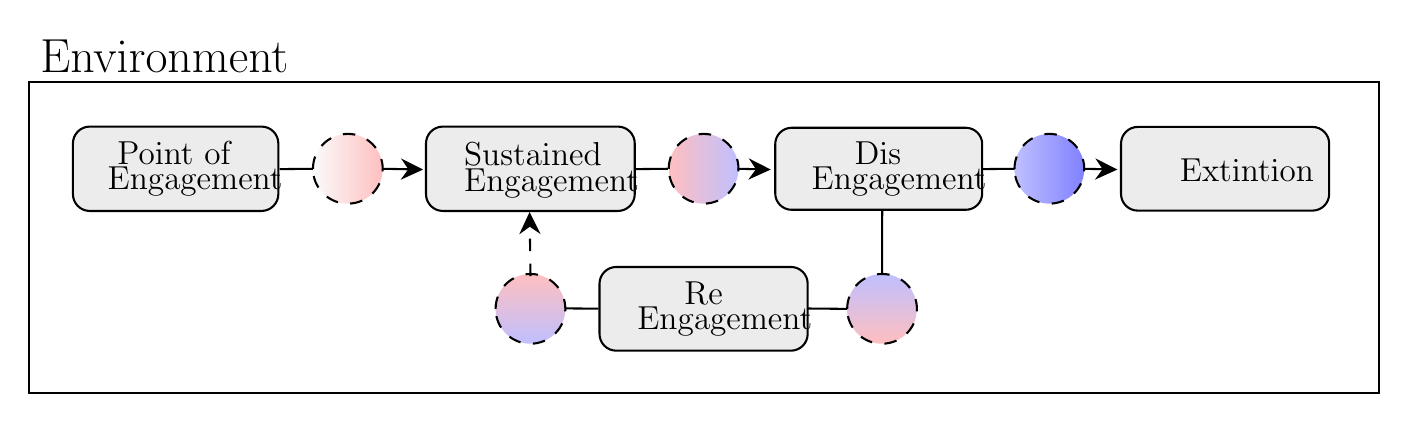
\begin{tikzpicture}[x=0.75pt,y=0.75pt,yscale=-1,xscale=1]
%uncomment if require: \path (0,357); %set diagram left start at 0, and has height of 357

%Rounded Rect [id:dp08887598870261693] 
\draw  [fill={rgb, 255:red, 236; green, 236; blue, 236 }  ,fill opacity=1 ] (30.4,81.08) .. controls (30.4,76.59) and (34.04,72.95) .. (38.53,72.95) -- (121.24,72.95) .. controls (125.73,72.95) and (129.37,76.59) .. (129.37,81.08) -- (129.37,105.48) .. controls (129.37,109.97) and (125.73,113.61) .. (121.24,113.61) -- (38.53,113.61) .. controls (34.04,113.61) and (30.4,109.97) .. (30.4,105.48) -- cycle ;
%Rounded Rect [id:dp06222122397376195] 
\draw  [fill={rgb, 255:red, 236; green, 236; blue, 236 }  ,fill opacity=1 ] (200.51,81.08) .. controls (200.51,76.59) and (204.16,72.95) .. (208.65,72.95) -- (292.95,72.95) .. controls (297.44,72.95) and (301.09,76.59) .. (301.09,81.08) -- (301.09,105.48) .. controls (301.09,109.97) and (297.44,113.61) .. (292.95,113.61) -- (208.65,113.61) .. controls (204.16,113.61) and (200.51,109.97) .. (200.51,105.48) -- cycle ;
%Rounded Rect [id:dp7821816318063516] 
\draw  [fill={rgb, 255:red, 236; green, 236; blue, 236 }  ,fill opacity=1 ] (368.77,81.42) .. controls (368.77,77.06) and (372.31,73.52) .. (376.68,73.52) -- (460.58,73.52) .. controls (464.95,73.52) and (468.49,77.06) .. (468.49,81.42) -- (468.49,105.14) .. controls (468.49,109.5) and (464.95,113.04) .. (460.58,113.04) -- (376.68,113.04) .. controls (372.31,113.04) and (368.77,109.5) .. (368.77,105.14) -- cycle ;
%Rounded Rect [id:dp20372970008362923] 
\draw  [fill={rgb, 255:red, 236; green, 236; blue, 236 }  ,fill opacity=1 ] (535.37,81.18) .. controls (535.37,76.73) and (538.98,73.12) .. (543.44,73.12) -- (627.59,73.12) .. controls (632.05,73.12) and (635.66,76.73) .. (635.66,81.18) -- (635.66,105.38) .. controls (635.66,109.83) and (632.05,113.44) .. (627.59,113.44) -- (543.44,113.44) .. controls (538.98,113.44) and (535.37,109.83) .. (535.37,105.38) -- cycle ;
%Shape: Circle [id:dp19552380180112794] 
\path  [shading=_j7rsmr3nr,_tol09vz9c,path fading= _y4z1b8bbb ,fading transform={xshift=2}] (146.05,93.28) .. controls (146.05,84) and (153.57,76.48) .. (162.85,76.48) .. controls (172.13,76.48) and (179.65,84) .. (179.65,93.28) .. controls (179.65,102.56) and (172.13,110.08) .. (162.85,110.08) .. controls (153.57,110.08) and (146.05,102.56) .. (146.05,93.28) -- cycle ; % for fading 
 \draw  [dash pattern={on 4.5pt off 4.5pt}] (146.05,93.28) .. controls (146.05,84) and (153.57,76.48) .. (162.85,76.48) .. controls (172.13,76.48) and (179.65,84) .. (179.65,93.28) .. controls (179.65,102.56) and (172.13,110.08) .. (162.85,110.08) .. controls (153.57,110.08) and (146.05,102.56) .. (146.05,93.28) -- cycle ; % for border 

%Shape: Circle [id:dp27430889542654724] 
\path  [shading=_2t0kw1fpw,_3ywdqyfah,path fading= _y32y00acn ,fading transform={xshift=2}] (317.46,93.28) .. controls (317.46,84) and (324.98,76.48) .. (334.26,76.48) .. controls (343.54,76.48) and (351.06,84) .. (351.06,93.28) .. controls (351.06,102.56) and (343.54,110.08) .. (334.26,110.08) .. controls (324.98,110.08) and (317.46,102.56) .. (317.46,93.28) -- cycle ; % for fading 
 \draw  [dash pattern={on 4.5pt off 4.5pt}] (317.46,93.28) .. controls (317.46,84) and (324.98,76.48) .. (334.26,76.48) .. controls (343.54,76.48) and (351.06,84) .. (351.06,93.28) .. controls (351.06,102.56) and (343.54,110.08) .. (334.26,110.08) .. controls (324.98,110.08) and (317.46,102.56) .. (317.46,93.28) -- cycle ; % for border 

%Rounded Rect [id:dp4578454458037269] 
\draw  [fill={rgb, 255:red, 236; green, 236; blue, 236 }  ,fill opacity=1 ] (284.11,148.66) .. controls (284.11,144.2) and (287.73,140.59) .. (292.18,140.59) -- (376.33,140.59) .. controls (380.79,140.59) and (384.4,144.2) .. (384.4,148.66) -- (384.4,172.85) .. controls (384.4,177.31) and (380.79,180.92) .. (376.33,180.92) -- (292.18,180.92) .. controls (287.73,180.92) and (284.11,177.31) .. (284.11,172.85) -- cycle ;
%Shape: Circle [id:dp8141702965644008] 
\path  [shading=_mzd6axxaa,_k82gbaai2,path fading= _wr0vkxl3y ,fading transform={xshift=2}] (484.05,93.28) .. controls (484.05,84) and (491.57,76.48) .. (500.85,76.48) .. controls (510.13,76.48) and (517.65,84) .. (517.65,93.28) .. controls (517.65,102.56) and (510.13,110.08) .. (500.85,110.08) .. controls (491.57,110.08) and (484.05,102.56) .. (484.05,93.28) -- cycle ; % for fading 
 \draw  [dash pattern={on 4.5pt off 4.5pt}] (484.05,93.28) .. controls (484.05,84) and (491.57,76.48) .. (500.85,76.48) .. controls (510.13,76.48) and (517.65,84) .. (517.65,93.28) .. controls (517.65,102.56) and (510.13,110.08) .. (500.85,110.08) .. controls (491.57,110.08) and (484.05,102.56) .. (484.05,93.28) -- cycle ; % for border 

%Shape: Circle [id:dp5389996328417695] 
\path  [shading=_wvh4fdo7p,_3kvg59946,path fading= _tndnn1d2b ,fading transform={xshift=2}] (234.05,160.76) .. controls (234.05,151.48) and (241.57,143.96) .. (250.85,143.96) .. controls (260.13,143.96) and (267.65,151.48) .. (267.65,160.76) .. controls (267.65,170.03) and (260.13,177.56) .. (250.85,177.56) .. controls (241.57,177.56) and (234.05,170.03) .. (234.05,160.76) -- cycle ; % for fading 
 \draw  [dash pattern={on 4.5pt off 4.5pt}] (234.05,160.76) .. controls (234.05,151.48) and (241.57,143.96) .. (250.85,143.96) .. controls (260.13,143.96) and (267.65,151.48) .. (267.65,160.76) .. controls (267.65,170.03) and (260.13,177.56) .. (250.85,177.56) .. controls (241.57,177.56) and (234.05,170.03) .. (234.05,160.76) -- cycle ; % for border 

%Shape: Circle [id:dp655926787503073] 
\path  [shading=_f5gjc5tzr,_475pso13i,path fading= _wo5obn5gu ,fading transform={xshift=2}] (403.43,160.76) .. controls (403.43,151.48) and (410.95,143.96) .. (420.23,143.96) .. controls (429.51,143.96) and (437.03,151.48) .. (437.03,160.76) .. controls (437.03,170.03) and (429.51,177.56) .. (420.23,177.56) .. controls (410.95,177.56) and (403.43,170.03) .. (403.43,160.76) -- cycle ; % for fading 
 \draw  [dash pattern={on 4.5pt off 4.5pt}] (403.43,160.76) .. controls (403.43,151.48) and (410.95,143.96) .. (420.23,143.96) .. controls (429.51,143.96) and (437.03,151.48) .. (437.03,160.76) .. controls (437.03,170.03) and (429.51,177.56) .. (420.23,177.56) .. controls (410.95,177.56) and (403.43,170.03) .. (403.43,160.76) -- cycle ; % for border 

%Shape: Rectangle [id:dp8053989914309859] 
\draw   (9.1,51.6) -- (659.6,51.6) -- (659.6,201.3) -- (9.1,201.3) -- cycle ;
%Straight Lines [id:da46348057228029615] 
\draw    (130,93.45) -- (146.05,93.28) ;
%Straight Lines [id:da06616438858203633] 
\draw    (179.65,93.28) -- (196.1,93.59) ;
\draw [shift={(199.1,93.65)}, rotate = 181.09] [fill={rgb, 255:red, 0; green, 0; blue, 0 }  ][line width=0.08]  [draw opacity=0] (10.72,-5.15) -- (0,0) -- (10.72,5.15) -- (7.12,0) -- cycle    ;
%Straight Lines [id:da6977755883492565] 
\draw    (350.65,93.28) -- (363.6,93.58) ;
\draw [shift={(366.6,93.65)}, rotate = 181.33] [fill={rgb, 255:red, 0; green, 0; blue, 0 }  ][line width=0.08]  [draw opacity=0] (10.72,-5.15) -- (0,0) -- (10.72,5.15) -- (7.12,0) -- cycle    ;
%Straight Lines [id:da47311877150256343] 
\draw    (301,93.45) -- (317.05,93.28) ;
%Straight Lines [id:da21451072469562127] 
\draw    (468,93.45) -- (484.05,93.28) ;
%Straight Lines [id:da7997515132020875] 
\draw    (517.65,93.28) -- (530.6,93.58) ;
\draw [shift={(533.6,93.65)}, rotate = 181.33] [fill={rgb, 255:red, 0; green, 0; blue, 0 }  ][line width=0.08]  [draw opacity=0] (10.72,-5.15) -- (0,0) -- (10.72,5.15) -- (7.12,0) -- cycle    ;
%Straight Lines [id:da5942266070774226] 
\draw    (420.23,143.98) -- (420.32,112.84) ;
%Straight Lines [id:da1853788628800106] 
\draw  [dash pattern={on 4.5pt off 4.5pt}]  (250.85,144.98) -- (250.47,117.1) ;
\draw [shift={(250.42,114.1)}, rotate = 89.2] [fill={rgb, 255:red, 0; green, 0; blue, 0 }  ][line width=0.08]  [draw opacity=0] (10.72,-5.15) -- (0,0) -- (10.72,5.15) -- (7.12,0) -- cycle    ;
%Straight Lines [id:da47123825108915496] 
\draw    (403.43,160.78) -- (384.32,160.6) ;
%Straight Lines [id:da3253725947262416] 
\draw    (283.52,160.68) -- (267.65,160.55) ;

% Text Node
\draw (334.26,160.76) node  [font=\fontsize{0.67em}{0.8em}\selectfont] [align=left] {\begin{minipage}[lt]{47.87pt}\setlength\topsep{0pt}
\begin{center}
{\large Re}\\{\large Engagement}
\end{center}

\end{minipage}};
% Text Node
\draw (79.09,93.28) node  [font=\fontsize{0.67em}{0.8em}\selectfont] [align=left] {\begin{minipage}[lt]{47.87pt}\setlength\topsep{0pt}
\begin{center}
{\large Point of}\\{\large Engagement}
\end{center}

\end{minipage}};
% Text Node
\draw (60.5,38.28) node  [font=\fontsize{0.67em}{0.8em}\selectfont] [align=left] {\begin{minipage}[lt]{68.75pt}\setlength\topsep{0pt}
\begin{center}
{\LARGE Environment}
\end{center}

\end{minipage}};
% Text Node
\draw (418.23,93.28) node  [font=\fontsize{0.67em}{0.8em}\selectfont] [align=left] {\begin{minipage}[lt]{47.87pt}\setlength\topsep{0pt}
\begin{center}
{\large Dis}\\{\large Engagement}
\end{center}

\end{minipage}};
% Text Node
\draw (585.51,93.28) node  [font=\fontsize{0.67em}{0.8em}\selectfont] [align=left] {\begin{minipage}[lt]{32.64pt}\setlength\topsep{0pt}
\begin{center}
{\large Extintion}
\end{center}

\end{minipage}};
% Text Node
\draw (250.8,93.28) node  [font=\fontsize{0.67em}{0.8em}\selectfont] [align=left] {\begin{minipage}[lt]{47.87pt}\setlength\topsep{0pt}
\begin{center}
{\large Sustained}\\{\large Engagement}
\end{center}

\end{minipage}};
\end{tikzpicture}

\end{adjustbox}
\end{center}
\caption{\textbf{Diagram summarizing the different stages of the engagement process model introducing the contribution of the individual's motivational state}. Solid and dashed lines represent observable and unobservable element in the process. The description of the process is the same as described in Figure \ref{fig: eng_proc_model_1} but the transition between observable engagement stages is controlled by a latent variable defining the motivational propensity of the individual towards the object they are engaging with.}
\label{fig: eng_proc_model_2}
\end{figure}